\documentclass[crop,tikz]{standalone}
\usepackage{pgfplots}
\pgfplotsset{compat=1.13}

% Field lines and lines of constant potential for a cylinder of radius
% 1/4 at position z = 1/2 inside a second cylinder of radius 1 at
% position z = 0.
%
% Inspired by the expressions given Arens, chapter 32.2.

\pgfplotsset{
  inverted/.style = {
    every axis legend/.append style={
      draw=white,
      fill=hardblack,
      text=white
    }
  },
  every non boxed x axis/.append style={
    axis line style={-latex}
  },
  every non boxed y axis/.append style={
    axis line style={-latex}
  }
}

\begin{document}

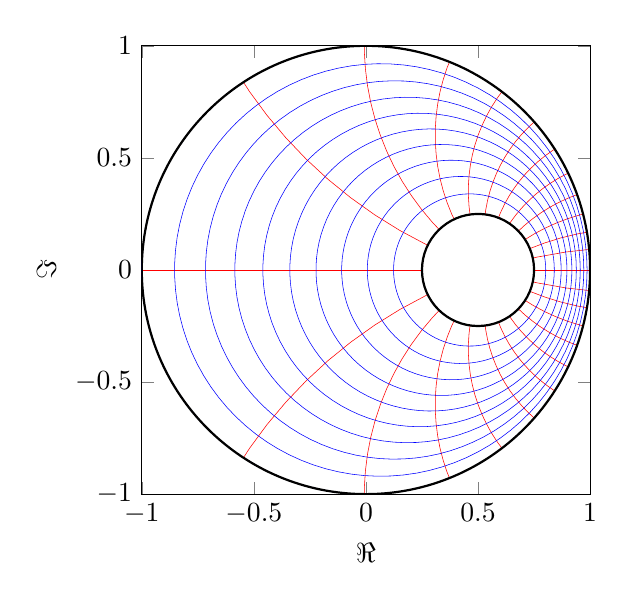
\begin{tikzpicture}
  \pgfmathsetmacro{\numberofpotentiallines}{10};
  \pgfmathsetmacro{\numberoffieldlines}{10};
  \pgfmathsetmacro{\xoff}{0.5}; % x coordinate of inner cylinder
  \pgfmathsetmacro{\zo}{(19 - sqrt(105))/16};
  \pgfmathsetmacro{\rmin}{1/4}; % radius of inner cylinder
  \pgfmathsetmacro{\rmax}{1}; % radius of outer cylinder
  \pgfmathsetmacro{\remin}{-1};
  \pgfmathsetmacro{\remax}{-\remin};
  \pgfmathsetmacro{\immin}{-1};
  \pgfmathsetmacro{\immax}{-\immin};
  \begin{axis}[
    axis equal image,
    xmin={\remin}, xmax={\remax},
    ymin={\immin}, ymax={\immax},
    xlabel={$\Re$},
    ylabel={$\Im$},
    samples=100,
    domain=0:360,
    declare function = {
      % lines of constant potential
      phixo(\c,\zo) = \zo*(1 - \c)/(1 - \c*\zo^2); % x-shift
      phir(\c,\zo) = sqrt(\c)*(1 - \zo^2)/(1 - \c*\zo^2); % radius
      phix(\x,\c,\zo) = phir(\c,\zo)*cos(\x) + phixo(\c,\zo); % x coordinate
      phiy(\x,\c,\zo) = phir(\c,\zo)*sin(\x); % y coordinate
      % electric field lines
      Er(\p,\zo) = (1 - \zo^2)/(2*sin(\p)*\zo); % radius
      Exo(\zo) = (1 + \zo^2)/(2*\zo); % x-shift
      Eyo(\p,\zo) = -(1 - \zo^2)/(2*tan(\p)*\zo); % y-shift
      Ex(\x,\p,\zo) = Er(\p,\zo)*cos(\x) + Exo(\zo); % x coordinate
      Ey(\x,\p,\zo) = Er(\p,\zo)*sin(\x) + Eyo(\p,\zo); % y coordinate
      % helper functions to calculate parameter ranges
      sqrtc(\r,\zo,\s) = -(1 - \zo^2)/(2*\r*\zo^2) + \s*sqrt(((1 - \zo^2)/(2*\r*\zo^2))^2 + 1/\zo^2); % sqrt(c) as a function of the radius r
      cmin(\zo) = sqrtc(\rmin,\zo,1)^2; % minimum c
      cmax(\zo) = sqrtc(\rmax,\zo,1)^2; % maximum c
      fc(\n,\nmax) = cmin(\zo) + \n/\nmax*(cmax(\zo) - cmin(\zo)); % calculates c
      pc(\n,\nmax) = 180/\nmax*(1 + \n/\nmax*(\nmax - 2)); % calculates phase
    },
    ]
    \begin{scope}[even odd rule]
      \clip (0,0) circle ({\rmax}) ({\xoff},0) circle ({\rmin});
      % field lines
      \pgfplotsinvokeforeach{0,...,{\numberoffieldlines}}{
        \addplot[red,very thin,domain=0:360] (
          {Ex(x, pc(#1,\numberoffieldlines), \zo)},
          {Ey(x, pc(#1,\numberoffieldlines), \zo)}
          );
      }
      \draw[red,very thin] ({-\rmax},0) -- ({\xoff-\rmin},0) ({\xoff+\rmin},0) -- ({\rmax},0);
      % lines of constant potential
      \pgfplotsinvokeforeach{0,...,{\numberofpotentiallines}}{
        \addplot[blue,very thin] (
          {phix(x, fc(#1,\numberofpotentiallines), \zo)},
          {phiy(x, fc(#1,\numberofpotentiallines), \zo)}
        );
      }
    \end{scope}
    % zylindric capacitors
    \draw[thick] (0,0) circle ({\rmax});
    \draw[thick] ({\xoff},0) circle ({\rmin});
  \end{axis}
\end{tikzpicture}
\end{document}
